% !TEX root = ../thesis.tex

\chapter{Využitie technologií v praxi}
\label{methodology}

Na vyriešenie problematiky nasadenia strojového učenia na platforme Kubernetes sú v tejto časti poskytnuté postupy na lokálne nasadenie na zariadeniach ako je laptop alebo stolný počítač. Jedna sa prevažne o platformu Kubeflow. Riešenia, ktoré sú poskytnuté sú mierne hardverovo záťažové, čo znamená, že sú vhodné pre zariadenia s hardvérovým vybavením minimálne 2 GB veľkou operačnou pamäťou a s voľným priestorom na disku. Dodané postupy sú vhodné, či už pre slabšie zariadenia ale aj výkonovo silnejšie pre plné nasadenie platformy.

\section{Kubeflow}
Kubeflow ako platforma, je vhodná na nasadenie a vývoj strojového učenia. Primárne slúži pre inžinierov a vedcov, ktorý pracujú s dátami. Obsahuje viaceré komponenty, z ktorých si vývojári môžu vybrať, čo je pre ich používateľov najlepšie, čo znamená, že na nasadzovanie nie je potrebný každý jeden komponent.

\subsection{Komponenty}

Stavia na platforme Kubernetes ako systéme na nasadenie, škálovanie a správu zložitých systémov. Pomocou konfiguračných rozhraní Kubeflow, môžeme špecifikovať nástroje strojového učenia, potrebné pre náš pracovný postup. Potom môžeme nasadiť pracovný postup do rôznych cloudov, miestnych platforiem na experimentovanie a na produkčné použitie.

V tejto časti sú priblížené všetky šesť komponenty, ktoré tvoria Kubeflow.


\subsection*{Pipelines}

Pipelines sa používajú na vytváranie a nasadzovanie prenosných, škálovateľných, pracovných postupov strojového učenia založených na kontajneroch Docker. Pozostávajú z používateľského rozhrania na správu tréningových experimentov, úloh a chodov a z nástroja na plánovanie viackrokových pracovných postupov strojového učenia. Existujú aj dve súpravy SDK, jedna umožňuje definovať a manipulovať s pipelines, zatiaľ čo druhá ponúka alternatívny spôsob interakcie Notebookov so systémom \cite{pipe}.

\subsection*{Notebooks}

Jupyter notebooks fungujú s Kubeflow veľmi dobre, pretože sa dajú ľahko integrovať s typickými mechanizmami overovania a kontroly prístupu. Používatelia môžu bezpečne a s istotou vytvárať notebookové moduly/servery priamo v klastri Kubeflow pomocou obrazov poskytnutých správcami a jednoducho odosielať úlohy s jedným uzlom v porovnaní s tým, že si musia všetko nakonfigurovať na svojom laptope.


\subsection*{Katib}

Katib je škálovateľný a rozšíriteľný framework, ktorý podporuje ladenie hyperparametrov a vyhľadávanie neurónovej architektúry. Umožňuje používateľom objaviť modely, ktoré sú rovnako dobré ako ručne vytvorené modely, bez toho, aby museli prejsť namáhavým manuálnym procesom konfigurácie a opakovania. Katib organizuje optimalizáciu alebo vyhľadávanie neurónovej architektúry a presúva ju do sekcie s názvom Experiment. Algoritmy bežia interaktívnym spôsobom. Experiment definuje vyhľadávací priestor, cieľ metrík a maximálny počet iterácií. Katib hľadá iteratívne vo vyhľadávacom priestore, aby splnil cieľ metrík alebo aby dosiahol maximálny počet opakovaní. Katib podporuje dva rôzne mechanizmy – Hyperparameter Tuning a Neural Architecture Search \cite{katib}.

Ladenie hyperparametrov je proces optimalizácie hodnôt hyperparametrov modelu s cieľom maximalizovať predikčnú kvalitu modelu. Príkladmi takýchto hyperparametrov sú rýchlosť učenia, hĺbka neurálnej architektúry (vrstvy) a šírka (uzly), epochy, veľkosť dávky, miera výpadkov a aktivačné funkcie. Toto sú parametre, ktoré sa nastavujú pred tréningom; na rozdiel od parametrov modelu (váhy a odchýlky) sa tieto nemenia počas procesu trénovania modelu.

\subsection*{Training operators}

Operátor Kubeflow pomáha nasadzovať, monitorovať a spravovať životný cyklus Kubeflow. Je zložený z Operator frameworku, čo je súprava nástrojov s otvoreným zdrojovým kódom na zostavovanie, testovanie, balenie operátorov a správu životného cyklu operátorov. Operátor Kubeflow používa KfDef ako svoj vlastný zdroj a kfctl ako základný nástroj na spustenie operátora.

Napríklad operátor k8s spadá pod Kubeflow. Tento operátor uľahčuje spúšťanie úloh tensorflow, či už sú distribuované alebo nedistribuované na kubernetes. TFjobs sú vlastným zdrojom Kubernetes, ktorý sa používa na trénovanie alebo spustenie úloh trénovania na Kubernetes. Kubeflow udržiava všetky tieto operátory a dá sa povedať, že Kubeflow zhromažďuje také komponenty, ktoré uľahčujú spustenie kódu strojového učenia v rôznych formách v rámci Kubernetes. Takže potrebný je operátor pre TFJob, ktorý to bude monitorovať a sledovať. Nasadenie Kubeflow, dokáže rozšíriť nasadenia operátorov, a potom podľa toho definovať TFjobs a spustiť toľko, koľko tréningov je potrebné na klastri kubernetes \cite{operator}.

\subsection*{Multi-Tenancy}

Po nainštalovaní a nakonfigurovaní Kubeflow sa predvolene pristupuje k primárnemu profilu. Profil vlastní menný priestor Kubernetes s rovnakým názvom spolu s kolekciou zdrojov Kubernetes. Používatelia majú prístup na zobrazenie a úpravu svojich primárnych profilov. Prístup k profilu je možné zdieľať s iným používateľom v systéme. Pri zdieľaní prístupu k profilu je na výber, aký prístup je možné poskytnúť na čítanie alebo prístup na čítanie/úpravu. Na všetky praktické účely pri práci s centrálnym ovládacím panelom Kubeflow je aktívny menný priestor priamo prepojený s aktívnym profilom.

\subsection*{Rozhranie}

Centrum riadenia komponentov, ktoré poskytuje používateľovi prístup k jednotlivým komponentom v klastri ako sú Pipelines, Notebooks, Katib, Artifact store a Multi-Tenancy.

Na nasledujúcom obrázku je možné vidieť rozhranie a niektoré komponenty, ktoré kubeflow ponúka.

\clearpage

\begin{figure}[h!]
    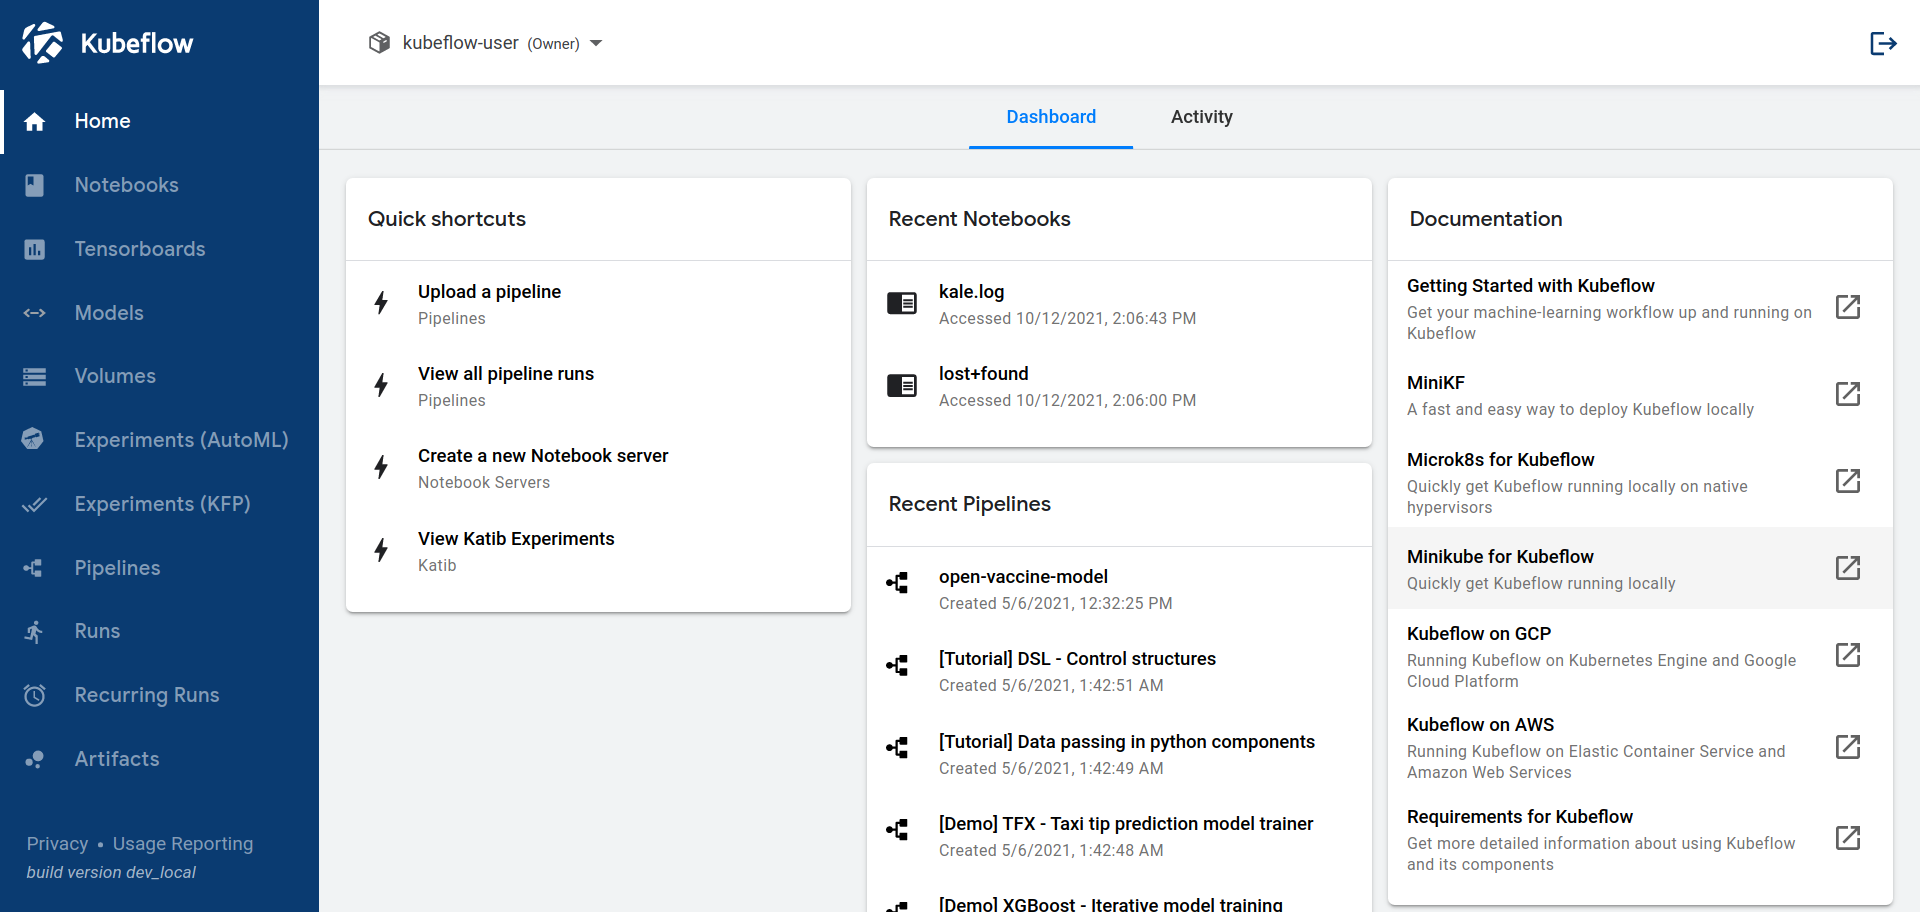
\includegraphics[width=\linewidth]{figures/Rozhranie}
    \caption{ Rozhranie Kubeflow }
\end{figure}

\subsection{Pracovný postup}

Postup pozostáva z viacerých krokov, taktiež z iterácie, ktorá je hlavným prvkom pri vyvíjaní sýtemu strojového učenia. Pri tomto postupe je potrebné vykonávať zmeny v parametroch aby sme dosiahli požadované výsledky. Následne si povieme niečo viac o týchto postupoch.

Ako prvé by sme mali vyvíjať model na základe predpokladov a testov. Môžeme ho opísať v nasledujúcich bodoch: \cite{work}

\begin{itemize}
    \item Identifikovanie problému, ktorý ma systém vyriešiť.
    \item Zbieranie dát, ktoré potrebujeme na trénovanie modelu.
    \item Vyberanie algoritmu a nakódovanie modelu.
    \item Experiment s údajmi a trénovanie modelu.
	\item Vyladenie parametrov.
\end{itemize}

Ďalej môžeme nasadiť systém, ktorý bude vykonávať tieto procesy:

\begin{itemize}
    \item Transformáciu údajov, ktoré náš systém potrebuje.
	\item Trénovanie modelu.
	\item Podanie modelu na online prevádzku.
	\item Monitorovanie výsledkov na úpravu a zmenu modelu.
\end{itemize}

\begin{figure}[!ht]
    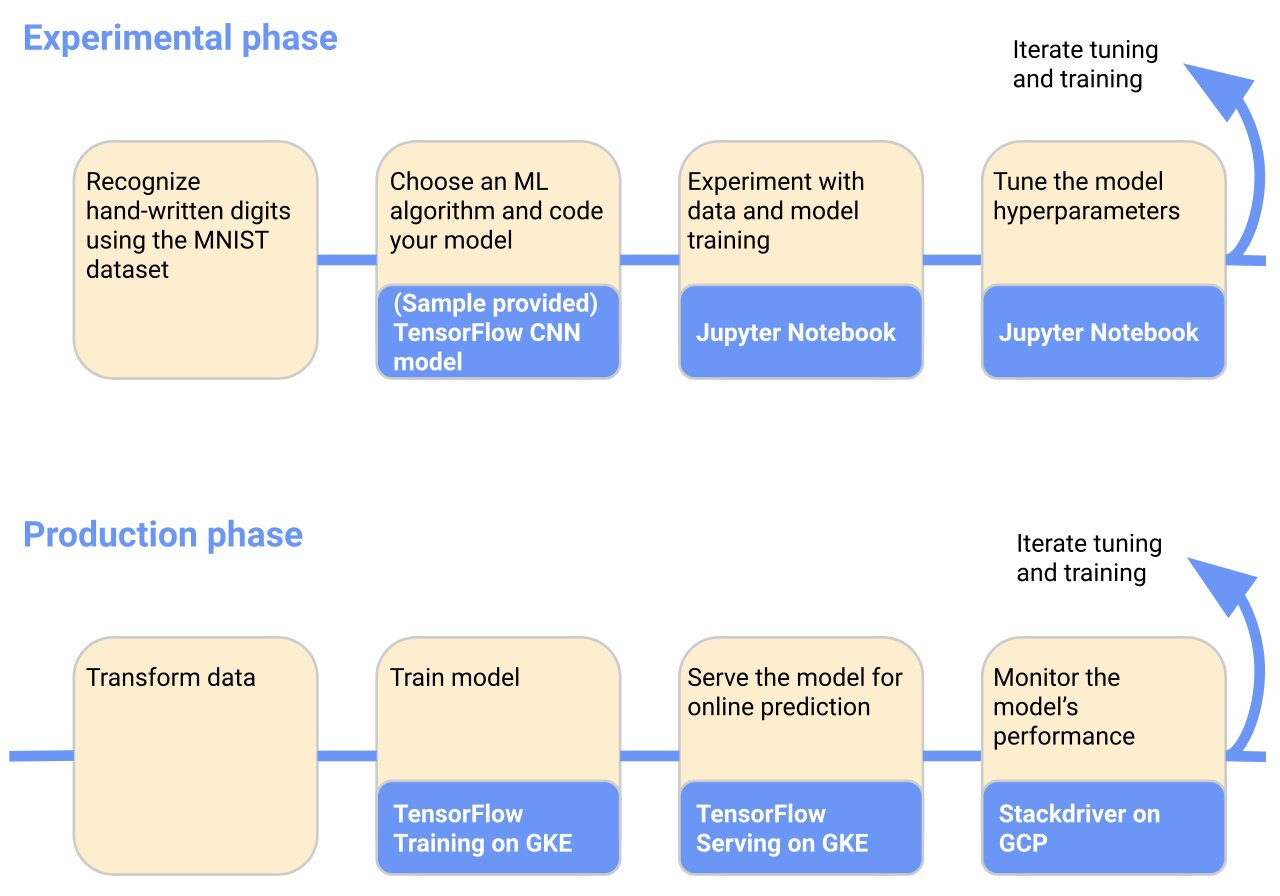
\includegraphics[width=.9\textwidth]{figures/kubeflowwork}
    \caption{\ Pracovné postupy \cite{work} \label{o:latex_friendly_zone}}
\end{figure}

\section{MiniKF}

Je softvér, vyvinutý spoločnosťou Arrikto, a to kombináciou viacerých služieb a nástrojov potrebných na spustenie úloh strojového učenia lokálne alebo vzdialene na platforme Kubernetes. Skladá sa z nástroja minikube na spustenie lokálnej platformy Kubernetes, samotného Kubeflow a platformy Rok, ktorá umožňuje spúšťanie stavových kontajnerov cez rýchle lokálne úložisko NVMe. MiniKF je lokálne nasadenie Kubeflow, ktoré je možné nainštalovať v priebehu minút. Po niekoľkých kliknutiach je možné začať experimentovať a dokonca spúšťať Machine Learning Pipelines.

Pred inštaláciou je potrebné nainštalovať VirtualBox a Vagrant. Je to softvér na vytváranie a udržovanie prenosných prostredí. Pre lokálne spustenie MiniKF je potrebné spĺňať minimálne požiadavky pre operačnú pamäť minimálne 12 GB, 2 jadra procesora a 50 GB voľného miesta na disku. Na operačnom systéme nezáleží, pretože je ho možné virtualizovať na rôznych operačných systémoch napríklad ako je Linux, macOS a Windows.

Inštalácia prebieha jednoducho a pozostáva z dvoch príkazov. Prvým príkazom sa stiahne konfiguračný súbor alebo obraz do daného priečinka a inicializujeme virtuálny počítač.
\begin{lstlisting}[language=Bash]
    $ vagrant init arrikto/minikf
    \end{lstlisting}
Druhým príkazom sa zapne virtuálny počítač a spustí sa konfiguračný súbor.
\begin{lstlisting}[language=Bash]
    $ vagrant up
    \end{lstlisting}
Kubeflow je poháňaný prostredníctvom Kubernetes na tomto virtuálnom počítací. Ak je virtuálny počítač pripravený spusti sa na ňom skript a následne je možné sa pripojiť cez internetový prehliadač na adrese 10.10.10.10 k danému počítaču, kde sa spustí nástroj, ktorý developuje serie softvérových balíčkov potrebných na spustenie Kubeflow. Po reštartovaní počítača sa dáta nestratia, stačí zopakovať postup a je možné sa vrátiť k začatej práci.

\section{Charmed}

Pri developovaní Kubeflow sa pri tomto spôsobe využíva Juju Charm. Juju Charm je bezplatný aplikačný nástroj na modelovanie aplikácii s otvoreným zdrojovým kódom vyvinutý spoločnosťou Canonical, je známy aj ako štruktúrovaný balík konfiguračných súborov YAML a skriptov pre softvérový komponent, ktorý umožňuje Juju nasadiť a spravovať softvérový komponent ako službu podľa osvedčených postupov. Poskytuje centrálny pohľad na operátorov Kubernetes v nasadení, konfigurácií, rozsahu a stavu každého z nich a integračných liniek medzi nimi. Sleduje potenciálne aktualizácie a inovácie pre každého operátora a koordinuje tok udalostí a správ medzi operátormi.

Tento spôsob je vhodný najmä pre používateľov s operačným systémom Ubuntu. Samozrejme ho je možné použiť aj na iných operačných systémoch použitím virtualizácie, odporúča sa využiť Multipass, nenáročného správcu virtuálnych počítačov Ubuntu. Poskytuje virtualizáciu využitím Hyper-V alebo VirtualBoxu. Minimálne požiadavky závisia od verzie Kubeflow a to pri verzii full sú väčšie, minimálne 16 GB operačnej pamäte a 60 GB voľného miesta na disku. Full verzia poskytuje všetky služby napríklad Katib a Jupyter Notebooks. Verzia s označením lite bola vytvorená pre používateľov, ktorí pracujú v prostredí s obmedzenými zdrojmi a mal by fungovať dobre pri 8 GB operačnej pamäte a 50 GB dostupných na disku. Zachováva užívateľsky dashboard, ktorý je vhodný najmä pre začiatočníkov s lepšou interakciou. Tento balík je orientovaný najmä na nasadenie na systémoch ako notebook. Poslednou a najľahšou verziou je edge, ktorá neobsahuje dashboard a je vhodná pre tých, ktorí vyžadujú vlastných operátorov alebo pre zariadenia so slabšími výkonom. Na spustenie postačuje 4 GB operačnej pamäte. Pri každej verzii sú potrebné 4 jadra procesora. Je možné tieto verzie aj editovať, ak neobsahujú niečo potrebné a to upravením YAML súboru.

Prvým krokom je nainštalovať Multipass, ak postup sa vykonáva na zariadení, ktorý ma operačný systém iný ako Ubuntu. Pre správne fungovanie sa využíva MicroK8s pre spravovanie klastra s 1.21 verziou Kubernetes. Je dostupná aj novšia verzia s označením 1.22, ktorá zatiaľ nepodporuje Kubeflow. Aby ďalšie príkazy fungovali bez použitia sudo je treba pridať používateľa do skupiny. Ak je Kubernetes pripravený, dostupné sú viaceré služby. Aby sa navzájom našli aplikácie, úložisko, prístup ku komponentom Kubeflow a aplikácii na vyrovnávanie záťaže MetalLB je nutné pridať DNS službu. Pred ďalšími krokmi sa kontroluje, či boli služby povolené. Pre developovanie Kubeflow platformy je nevyhnutný Juju nastroj. Jeho inštalácia je pomerne jednoduchá, pretože sa inštaluje z balíka využitím systému snap na spravovanie balíčkov. Spustenie príkazu na nasadenie ovládača Juju do Kubernetes pre ovládanie komponentov Kubeflow a odporúča sa taktiež nastaviť špecificky model. Po Juju nasleduje proces nasadenia Kubeflow a je treba vyčkať pokiaľ sa jednotlivé aplikácie a komponenty pripravia a budú môcť medzi sebou komunikovať. Pre prístup k dashboardu nakonfigurovanie niektorých komponentov je nevyhnutné s povolenou adresou URL. K dispozícii je aj možnosť nastavenia mena a hesla. Na záver je možné zobraziť dashboard v prehliadači s URL, ktorú sme nakonfigurovali. Ak sa využíva Multipass pre získanie prístupu je vhodné vytvoriť pripojenie použitím SSH so zapnutým SOCKS proxy.

\subsection{Pripojenie strojov do klastra}

Pridanie viacero uzlov (strojov) do klastra Kubernetes znamená, že pracovné zaťaženie môže byť rozdelené medzi rôzne uzly, ktoré sa môžu škálovať podľa ich špecifického zaťaženia. Nasadenia viacerých klastrov sú rozdelené do viacerých uzlov a škálujú sa podľa zaťaženia konkrétneho klastra. Čím drasticky znižuje spotrebu zdrojov jedného uzla a vedie k menšiemu zaťaženiu backendových služieb, ako sú databázy. Na rozdiel od modelu s jedným klastrom, prevádzkovanie v pracovných zaťažení poskytuje tvrdú úroveň izolácie. Riziko vzájomnej interakcie aplikácií alebo aplikácií s viacerými prostrediami, neúmyselným spôsobom je výrazne nižšie. Poskytuje lepši výkon poprepájaním strojov, ktorý je veľmi dôležitý pri strojovom učení. V tomto prípade je podstatnejší viacuzlový klaster než jednouzlový, najmä kvôli tomu, ak niektorý z hlavných uzlov zlyhá, ostatné uzly udržia klaster v prevádzke. Preto je vhodné vytvorenie viacuzlového klastra pripojením ďalších uzlov.

Postup je odlišný len na základe operačných systémov v ktorých sa bude pripájanie vykonávať. Požiadavky podľa oficiálnej dokumentácie sú nasledovné:

\begin{itemize}
    \item Každý uzol v klastri by mal mať aspoň 2GB pamäte RAM a 2 jadra procesora.
    \item Samozrejmosťou je verejné alebo súkromné sieťové pripojenie pre všetky stroje v klastri.
    \item Názov hostiteľa a MAC adresa musia byť jedinečné.
    \item Funkcia swap space, ktorá slúži na rozšírenie RAM pamäte na linuxových distribúciách musí byť vypnutá.
    \item Každý uzol vyžaduje svoje vlastné plne izolované prostredie - samostatný fyzický počítač, virtuálny stroj, kontajner alebo iný počítač v rovnakej sieti. V jednom prostredí nie je možné spustiť dve pracovné inštancie.
\end{itemize}

\subsection*{Linux/Ubuntu}

Ako prvé je potrebné spustiť tento príkaz na počítací, ktorý chceme aby bol riadiacim klastrom a zároveň hostiteľom riadiacej roviny Kubernetes.

\begin{lstlisting}[language=Bash]
    $ microk8s add-node
    \end{lstlisting}

Príkaz vygeneruje link s pokynmi na dočasnú registráciu pre nový uzol. V pokynoch sú príkazy, ktorými je možne vykonať spojenie uzla s riadiacou rovinou. Jeden z týchto príkazov sa spúšťa na stroji, ktorý chceme spojiť s uzlom, na ktorom bol spustení predošli príkaz. Proces pripojenia trvá niekoľko sekúnd. Pokyny su názorne ukázané na nasledujúcom obrázku.

\begin{figure}[h!]
    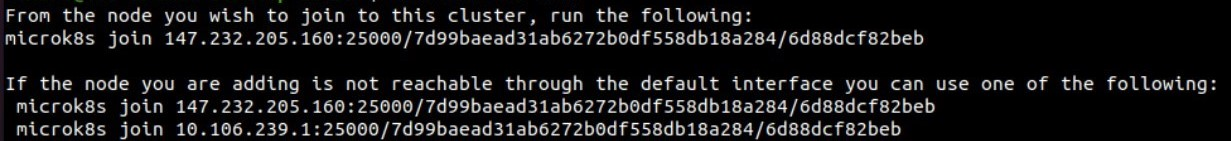
\includegraphics[width=\linewidth]{figures/addnode}
    \caption{ Príkazy na pripojenie stroja do klastra }
\end{figure}

Po pridaní uzla je možné hostiť pody na viacerých strojoch. Všetky dostupné uzly sa zobrazujú spustením príkazu:

\begin{lstlisting}[language=Bash]
    $ microk8s kubectl get nodes
    \end{lstlisting}

\subsection*{Windows Server 2019 alebo novší}

Pre zlúčenie stroja s operačným systémom Windows je dôležitý Docker na správu kontajnerov a pripravený klaster s Calico CNI. Je to sieťovo kontajnerové rozhranie označované ako CNI, ktoré rieši množstvo sieťových požiadaviek napríklad komunikáciu medzi kontajnermi alebo externými službami. Zároveň sa vyžaduje aj inštalácia calicoctl, nástroj príkazového riadka pre spravovanie Calico a vykonávanie administratívnych funkcii.

Pre prístup do klastra sa vyžaduje kópia súboru kubeconfig. Pre pody na Windowse musí byť strictaffinity nastavená na hodnotu ako pravdivá, aby sa zabránilo požičiavaniu IP adries z uzlov Windowsu. Vhodné je sa ubezpečiť aká verzia Kubernetes je nasadená v klastri.

Ďalším krokom je inštalácia komponentov na stroji s operačným systémom Windows pomocou prostredia PowerShell spustený ako správca. Inštalácia pozostáva z vytvorenia priečinka, do ktorého uložíme predošlú kópiu súboru kubeconfig, inštalácie systému Calico a spustenia služby Kubernetes.

\subsection{Odpojenie stroja z klastra}

Zmazanie stroja z klastra je jednoduché a uskutočňuje sa pomocou dvoch príkazov. Príkazy sa použijú na stroji, ktorý ma byť odstránení z klastra.

Microk8s reštartuje riadiacu rovinu na uzle, ktorý sa ma vymazať. Tým obnoví operácie a stane sa osobitným klastrom. V pôvodnom klastri sa označí ako nedostupný a nebudú sa naň nasadávať nove operácie.
\begin{lstlisting}[language=Bash]
    $ microk8s leave
    \end{lstlisting}
Pre úplne vymazanie stroja zo zostávajúcich uzlov sa používa nasledujúci príkaz s jeho IP adresou:
\begin{lstlisting}[language=Bash]
    $ microk8s remove-node <node_IP>
    \end{lstlisting}
\subsection{Podpora grafickej karty}

Implementovanie grafickej karty do klastra Kubernetes je veľkou výhodou najmä kvôli výraznému skráteniu času na riešenie náročno výpočtových operácií. Je veľkou výhodou pri strojovom učení. Pridanie grafickej karty vykonáme prostredníctvom tohto príkazu.

\begin{lstlisting}[language=Bash]
    $ microk8s enable gpu
    \end{lstlisting}

Pre pridanie grafickej karty je potrebné splniť nasledujúce body:

\begin{itemize}
    \item Platforma Kubeflow verzia full alebo lite je spustená v Kubernetes klastri.
    \item Je dostupné pripojenie na internet.
    \item Bolo uskutočnené prihlásenie prostredníctvom Kubeflow dashboardu.
    \item V hardvérovom vybavení je dostupná grafická karta od spoločnosti AMD alebo NVIDIA.
\end{itemize}

Ak je grafická karta povolená a pridaná do klastra niektoré pracovné úlohy môžu ju požadovať nastavenim limitu napríklad ako nvidia.com/gpu: 1.

\subsection{High aviability}

\section{Pipelines}

Tento spôsob je vhodný, vtedy ak je žiadaná práca výhradne s Kubeflow pipelines. Cieľom je nasadiť pipelines na lokálnom klastri. Na nasadenie nie sú nutné žiadne virtualizačné programy a postup je v celku jednoduchý, pretože sú tým výnimočne. Kubeflow pipelines sú známe kontajnerizáciou, čo znamená, že bude sa používať Docker na vytváranie kontajnerov. Požiadavky na spustenie nie sú náročne, pre operačnú pamäť si vyžadujú minimálne 8 GB a 2 jadra procesora. Nástroj kind je kľúčový, slúži na vytvorenie lokálneho Kubernetes klastra využitím Dockera. Taktiež by bolo dobre poznamenať, že Docker vyžaduje Windows Subsystem for Linux (WSL), ktorý slúži pre natívny beh linuxových spustiteľných súborov v prostredí Windows. Pre správny postup inštalácie sa požaduje aj kubectl, ktorý sa používa na komunikáciu s klastrom vyžitím príkazového riadka a Git.

Na začiatok je potrebné nainštalovať nástroj kind. Inštalácia na operačnom systéme Windows je veľmi jednoduchá a pozostáva z niekoľko príkazov, pripadne je možné použiť Chocolatey, ktorý je vhodný na inštaláciu balíčkov na systéme Windows. Ďalším krokom je vytvorenie klastra príkazom “kind create cluster”.  Kind spusti klaster Kubernetes pomocou vopred vytvoreného obrazu. Samozrejmosťou je použitie vlastného obrazu. Nasadenie pipelines sa vykoná spustením príkazov, ktoré stiahnu všetko potrebné z gitu a treba počkať niekoľko minút pokiaľ prebehne nasadenie všetkých komponentov potrebných pre pipelines a následne posledným krokom je presmerovanie portov. Po presmerovaní je Kubeflow dostupný otvorením internetového prehliadača na adrese „http://localhost:8080/“.

\section{Kubeadm}

Pri tomto postupe sa využíva nástroj Kubeadm, ktorý bol zavedený pre vytváranie Kubernetes klastrov. Je vyvíjaný oficiálnou komunitou Kubernetes. Poskytuje minimalisticky systém, veľmi dobru portabilitu a lokálne nasadenie na strojoch, ako sú napríklad notebook, Raspberry PI a podobne. Znižuje zložitosť a uľahčuje nasadenie použiteľného klastra Kubernetes. Minimálne požiadavky pre funkčný beh Kubernetes sú 2 GB operačnej pamäte a dve jadra procesora pre jeden stroj. V prípade riešeného problému tejto bakalárskej práce sa vyžaduje kvôli nasadeniu Kubeflow viac zdrojov. Záleží to od faktorov ako počet komponentov, ktoré sú požadované, koľko strojov je pripojených v klastri a s akými zdrojmi. Pre vytváranie kontajnerov nasadenie pozostáva aj z inštalácie vhodnej kontajnerovej služby ako je Docker.

Inštalácia je vykonávaná na linuxovej distribúcii. Pred nastavením klastra prostredníctvom Kubeadm je potrebné povoliť prenos cez firewall prostredníctvom IPtables. Funkcia Swap je aj v tomto spôsobe zakázaná. Základnou požiadavkou je nejaký obraz kontajnera. Na výber sú viaceré služby ako containerd, CRI-O alebo Docker. Po úspešnom nastavení je dôležité povoliť služby využívajúce kontajnerizáciu v systéme. Nutné je konfigurovať Kubeadm, Kubelet a Kubectl na verziu 1.21, keďže Kubeflow je do tejto verzie podporovaný a musí sa striktne dodržať. Pre prevenciu, aby sa programy neaktualizovali sa musia označiť ako hold, čo zabraní samovoľnému aktualizovaniu na novšiu verziu. Nasleduje inicializácia klastra na počítací prostredníctvom Kubeadm, ktorý bude riadiacou rovinou v platforme Kubernetes. Po úspešnej inicializácii Kubeadm sa vypíše výstup s umiestnením súboru kubeconfig, ktorý využíva Kubectl na interakciu s klastrom a príkaz join s tokenom. Je dobré ho niekde uchovať alebo neskôr znova vypísať, pretože je potrebný pri pridávaní stroja. V predvolenom nastavení sa pody nenaplánujú na hlavnom uzle. Hlavný uzol sa môže použiť na nasadzovanie podov, ak sa označí ako pracovný uzol. Kubeadm nenakonfiguruje žiadny sieťový doplnok. Pre správne fungovanie sa nastavuje sieťový doplnok ako Calico.

Ak je všetko dobre nastavené, overiť sa to da prostredníctvom príkazu Kubectl na vypísanie počítačov v klastri, či je daný poctiac pripravený. Počítač musí byť v stave Ready, čo znamená, že je pripravený na ďalšie kroky nasadzovania. Vhodné je aj nasadenie UI dashboardu pre lepšiu interakciu používateľa s platformou.

Spustenie Kubeflow platformy sa realizuje manuálnou inštaláciou manifestov. Existujú aj rôzni distribútori ako Google, Amazon alebo IBM. Ich služby a ich realizácia je jednoduchšia, sú však spoplatnené. Kubeflow vyžaduje nastavenie Kubernetes s prednastaveným StorageClass a nástroja Kustomize, ktorý slúži na prispôsobovanie objektov pomocou jeho Kustomize súborov. Kubeflow s verziou 1.5 zatiaľ nie je kompatibilný s najnovšou verziou Kustomize, preto musí byť verzia 3.2. Do počítača si naklonujeme oficiálny git repozitár od spoločnosti Kubeflow. Sú dva spôsoby implementovania manifestov použitím jedného, kde sa použijú všetky existujúce komponenty alebo pomocou viacerých príkazov a to vlastným výberom komponentov, ktoré sa vyžadujú. Po niekoľkých minútach sú všetky komponenty pripravené. A posledným krokom ostáva zapnutie Dashboardu, kde používateľ môže naplno využívať komponenty.

\subsection{Pripojenie strojov do klastra}

Implementácia a požiadavky sú podobné ako pri predchádzajúcom pripájaní strojov do klastra využitím Charmed Kubeflow nasadenia.

\subsection*{Linux/Ubuntu}

Pre pripojenie linuxového stroja je nutné na ňom zopakovať niektoré inštalačné postupy, ktoré boli vykonané pri konfigurácii Kubernetes klastra:

\begin{itemize}
    \item Povolit prenos cez Firewall pomocou IPtables
    \item Zákaz funkcie Swap
    \item Docker
    \item Kubeadm, Kubelet, kubectl
\end{itemize}

Po týchto krokoch je možné použiť hore spomínaný príkaz join na pripojenie stroja do klastra.

\subsection*{Windows Server 2019 alebo novší}

Spustenie a spojazdnenie komponentov pre platformu Kubernetes na Windowse je obťažnejšie a môže byt problémové. Pre pridanie stroja s operačným systémom Windows do klastra, ktorý beží na Linuxe je na ňom treba vykonať doplnkové akcie.

Na stroji, ktorý nesie označenie hlavnej roviny sa stiahne Flannel manifest, v~ktorom sa upravia čísla portov, aby Linux spolupracoval s Flannelom v systéme Windows. Flannel sa používa na priraďovanie IP adries kontajnerom a pre komunikáciu medzi nimi. Editovanú konfiguráciu je možné aplikovať do klastra. Treba však aj tu poznamenať dodržanie verzii, aby súladili s verziou Kubernetes spustenej na klastri. Po chvíli sa vytvoria sieťové Flannelové moduly.

Na stroji s Windowsom, ktorý sa pridáva do klastra vykonáme inštaláciu Dockera s verziou Engine Enterprise a povolenie funkcie Hyper-V. Na rade sú Wins, Kubelet a Kubeadm, ktoré musia mať rovnakú verziu ako klaster Kubernetes. Ako posledná akcia, ktorá by sa mala vykonať je použitie príkazu join.

\subsection{Odpojenie stroja z klastra}

Odstránenie prebieha pomocou nástroja kubectl, použitím nasledovných príkazov na riadiacej rovine.

Označenie stroja ako neplánovateľný, aby sa zamedzilo pridávaniu nových podov.

\begin{lstlisting}[language=Bash]
    $ kubectl cordon <node_ID>
    \end{lstlisting}

Bezpečné odstránenie všetkých podov z uzla pred odstránením. Vysťahovanie kontajnerov, aby sa mohli ukončiť pody na stroji, ktorý sa odstraňuje. Ak všetko prebehne v poriadku, znamená to, že všetky pody boli bezpečne odstránené alebo presunuté.

\begin{lstlisting}[language=Bash]
    $ kubectl drain <node_ID>
    \end{lstlisting}

Následne je možné prejsť k odstráneniu všetkých údajov o danom stroji z klastra.

\begin{lstlisting}[language=Bash]
    $ kubectl delete node cmp<node_ID>
    \end{lstlisting}

\subsection{Podpora grafickej karty}

Pridanie grafickej karty sa sprostredkuje prostredníctvom grafických kariet od spoločnosti NVDIA a AMD. Podmienkou je mať nainštalované ovládače od grafických kariet.
Operácia aplikovania grafickej karty je vykonaná prostredníctvom príkazu s manifestom vo forme YAML súboru podľa toho o akú grafickú kartu ide.

\begin{lstlisting}[language=Bash]
    $ kubectl create -f <manifest>
    \end{lstlisting}

Ak sa jedná o grafickú kartu spoločnosti NVIDIA je nutné spraviť dodatočné opatrenia:

\begin{itemize}
    \item Vopred nainštalovaný nástroj pre kontajnery nvidia-docker s verziou 2.0.
    \item Kubelet musí používať Docker ako svoj kontajnerový obraz.
    \item Nvidia-container-runtime nakonfigurovaný ako predvolený runtime pre Docker namiesto runc.
\end{itemize}
